\documentclass{llncs}

\usepackage{amsmath,amssymb,amsfonts}
\usepackage{algorithm}
\usepackage{algorithmic}
\usepackage{graphicx}
\usepackage{xcolor}
\usepackage{tikz}
\usepackage{booktabs}
\usepackage{url}
\usetikzlibrary{shapes.geometric, arrows.meta, positioning, fit}

\pagestyle{empty}

\usepackage{enumitem}
\setlist[itemize]{topsep=2pt,itemsep=1pt,parsep=0pt}
\setlength{\textfloatsep}{8pt plus 2pt minus 2pt}
\setlength{\intextsep}{8pt plus 2pt minus 2pt}
\setlength{\abovecaptionskip}{4pt}
\setlength{\belowcaptionskip}{2pt}
\setlength{\emergencystretch}{1.5em}

\begin{document}

\title{Attribution Without Validation:\\ Measuring Downstream Bias
in Failure Attribution for Multi-Agent Text-to-SQL}

\titlerunning{Attribution Without Validation}

\author{Minh-Quang Nguyen \and Quang-Dai Tran}
\authorrunning{M.-Q. Nguyen and Q.-D. Tran}

\institute{Research Institute of Posts and Telecommunications,\\
Posts and Telecommunications Institute of Technology, Hanoi, Vietnam\\
\email{QuangNM.B23CC140@stu.ptit.edu.vn, daitq@ptit.edu.vn}}

\maketitle

\begin{abstract}
Multi-Agent Systems (MAS) reach strong end-to-end Text-to-SQL accuracy but
give little visibility into which stage failed. We contribute a diagnostic
framework, a perturbation benchmark, and a validation protocol applied to the
attribution heuristic itself. The framework centres on a Logging Matrix that
records 13 intermediate state variables across four stages (Intent, Schema,
Skeleton, Execution) and localises failures by backward state-differencing.
On $7{,}000$ Spider executions ($6{,}782$ completed) it attributes $27.20\%$ of
outcomes to skeleton defects, while execution errors fall to $0.29\%$ after
self-correction. We then score the heuristic on $398$ perturbation instances
whose stressed stage is fixed by construction, and the result is negative:
stage-level recall is $0\%$ for injected intent faults ($0/98$, $95\%$ CI
$[0,3.8\%]$) and for injected schema faults ($0/54$, CI $[0,6.6\%]$). The
labels are biased downstream: $151$ of the $152$ perturbations that induced a
failure were labelled \texttt{Skeleton} ($60.5\%$) or \texttt{Execution}
($38.8\%$), and we cannot detect a difference between the two injection
conditions ($\chi^2=0.001$, $p=0.97$). We therefore report the stage distribution as
\emph{framework-attributed} rather than as a pipeline property, and withdraw
the claim that skeleton reasoning is the dominant failure source. The zero
recall is a property of this heuristic on this pipeline, not of
state-differencing as a class. The transferable contribution is the
protocol: inject at known stages, score recall, and publish the confusion
matrix alongside any stage distribution.

\keywords{Text-to-SQL \and Multi-Agent Systems \and Failure Attribution \and
Attribution Bias \and Diagnostic Benchmark \and Negative Results}
\end{abstract}

\section{Introduction}
\label{sec:intro}

Large Language Models (LLMs) have improved Text-to-SQL, and Multi-Agent
Systems (MAS) that split the task into specialised agents for intent
understanding, schema linking, skeleton generation and execution reach strong
results on benchmarks such as Spider~\cite{yu_spider_2018}. High benchmark
accuracy, however, hides which agent erred and at which stage the error
emerged~\cite{huo_bird_interact_2026,zhu_scot2s_2025}. Self-correction
therefore stays largely blind: it relies on execution feedback that consumes
many tokens and produces superficial fixes~\cite{zhu_scot2s_2025}. Stage-aware
repair is the obvious remedy, but it presupposes something the literature has
not established: that the stage labels used to route repair are accurate.

This paper asks two questions. \textbf{RQ1}: what stage distribution does a
state-differencing heuristic report over a large MAS Text-to-SQL corpus?
\textbf{RQ2}: when the faulty stage is known by construction, how often does
that heuristic recover it? Prior work leaves the second question unasked, and
answering it changes how the first should be read.

We make three contributions. \textbf{(1)}~A \emph{Logging Matrix} that records
13 intermediate artifacts per run (parsed intent, filtered schema, SQL
skeleton, execution traces and more), so that pipeline states can be compared
to localise discrepancies. \textbf{(2)}~A \emph{perturbation benchmark} of 400
instances whose faulty stage is known by design: schema-proxy distractors
target schema linking, and synonym paraphrases target intent understanding.
\textbf{(3)}~A \emph{bias-measurement protocol} that turns this benchmark on
the heuristic itself. Applied to our own backward state-differencing
procedure, it yields a negative result that we report in full: stage recall is
$0\%$ on both perturbation families, almost every injected fault is blamed on
a downstream stage (Skeleton or Execution), and the label distributions of the
two injection conditions are indistinguishable. The finding characterises
\emph{this} heuristic on \emph{this} pipeline (Section~\ref{sec:limitations}).
We argue that this measurement should precede any published stage
distribution, including our own in Table~\ref{tab:failures}. Code, logs and
the benchmark are released at
\url{https://github.com/MinhQuang0611/MAS-FailureAttribution}.

Throughout, Execution Accuracy (EX) denotes whether the predicted query's
result set matches that of the gold query~\cite{yu_spider_2018}.
Section~\ref{sec:related} reviews related work, Section~\ref{sec:methodology}
presents the framework and its ordering bias, Section~\ref{sec:experiments}
reports the distribution and the measurement of the heuristic,
Section~\ref{sec:limitations} states the limitations, and
Section~\ref{sec:conclusion} concludes.

\section{Related Work}
\label{sec:related}

\noindent\textbf{Multi-agent Text-to-SQL.} DIN-SQL showed that decomposing the
task into schema linking, query classification and self-correction improves
accuracy by about 10 points over a single prompt~\cite{pourreza_din-sql_2023}.
Later systems specialise agents further for intent understanding, query
planning and SQL
generation~\cite{chaturvedi_sqlofthought_2025,wang_mac-sql_2025,cen_sqlfixagent_2025}.
These systems remain end-to-end black boxes: intermediate states are not
systematically logged, so it is unclear which agent introduced an
error~\cite{lei_spider2_2025}.

\noindent\textbf{Error analysis and self-correction.} Schema-linking and join
mistakes are reported to cause over 70\% of parsing
errors~\cite{zhu_scot2s_2025}, and Shen et al.\ catalogue 27 error types in 7
categories for in-context-learning pipelines~\cite{shen_icl_errors_2026}.
SCoT2S fixes errors iteratively at the SQL level~\cite{zhu_scot2s_2025}, EMLC
corrects across schema, skeleton and executability
layers~\cite{lei_emlc_2026}, DAC separates entity and skeleton
correction~\cite{wang_dac_2025}, and SelECT-SQL ensembles self-correcting
chains of thought~\cite{shen_select-sql_2024}. Most of these patch the final
SQL without tracing which agent produced the defect.

\noindent\textbf{Automated failure attribution.} Zhang et
al.~\cite{zhang2025which} introduced the Who\&When dataset and found that even the
strongest method names the faulty agent for only 53.5\% of failures and the
decisive step for 14.2\%. We read that figure as the more important result:
their benchmark reports how often attribution succeeds, whereas ours reports
what a heuristic does when it fails. For our heuristic the answer is not
random error but a consistent shift toward downstream stages, which can
manufacture an apparent bottleneck. Attribution heuristics are often validated
against labels derived from the same intermediate signals they consume, which
cannot expose a shared bias. Cemri et al.~\cite{cemri_mast_2025} build MAST, a
14-mode taxonomy of multi-agent failures grounded in 1{,}600 annotated traces
($\kappa=0.88$); their human annotation is exactly the independent ground
truth heuristic attribution lacks, and our perturbation benchmark is a cheaper
substitute for it, not an improvement. Inferring an upstream cause from its downstream
effect is also the classical \emph{fault localisation} problem of software
engineering, where single-pass scoring is complemented by repeated
intervention such as delta debugging~\cite{zeller_delta_debugging_2002}. That literature
anticipates our negative result; we claim novelty only for measuring the effect
in MAS Text-to-SQL.

\noindent\textbf{Diagnostic benchmarks.} Spider~\cite{yu_spider_2018} reports
execution accuracy and exact match but no signal about where a pipeline
failed. Robustness suites such as Dr.\,Spider's 17 perturbation
types~\cite{chang_drspider_2023}, Spider-Syn~\cite{gan_spider_syn_2021},
Solid-SQL~\cite{liu_solid-sql_2025} and SQL2NL~\cite{safarzadeh_sql2nl_2025}
expose brittleness but do not trace failures to stages. We combine targeted
perturbations with the Logging Matrix so that the stage-level annotation is
fixed at construction time rather than assigned post hoc.

\section{Methodology}
\label{sec:methodology}

\subsection{Pipeline and Error Taxonomy}

Following common practice~\cite{shen_icl_errors_2026}, the pipeline has four
stages, each handled by a dedicated agent. \textbf{Intent} parses the question
into entities, filter conditions, aggregations and temporal constraints,
producing a semantic representation rather than SQL. \textbf{Schema} maps
linguistic cues to schema elements and keeps only the tables and columns
needed~\cite{yang_sql_to_schema_2024}. \textbf{Skeleton} arranges the core
clauses (\texttt{SELECT}, \texttt{FROM}, \texttt{JOIN}, \texttt{WHERE},
\texttt{GROUP BY}, \texttt{ORDER BY}) with value
placeholders~\cite{lei_emlc_2026}. \textbf{Execution} fills in values, runs
the query and returns a result set or an engine error. Figure~\ref{fig:running_example}
traces one perturbed instance through these stages.

The error taxonomy assigns each failure to the stage where the fault first
appears~\cite{shen_icl_errors_2026}: \emph{Intent} (missing condition,
misread operator); \emph{Schema} (missing table or column, hallucinated
element~\cite{chang_drspider_2023,lei_emlc_2026}); \emph{Skeleton} (wrong join,
wrong aggregation or grouping, malformed
subquery~\cite{chen_error_detection_2023}); and \emph{Execution} (syntax error,
type mismatch, or a valid query returning a wrong or empty result).

\begin{figure}[t]
    \centering
    \resizebox{0.96\textwidth}{!}{% running_example.tex — Figure 1
% LNCS copy for soict2026_logging.tex (labels moved to avoid overlaps).
% Included from conference_101719.tex via % running_example.tex — Figure 1
% Included from conference_101719.tex via % running_example.tex — Figure 1
% Included from conference_101719.tex via \input{running_example}
% Requires: \usetikzlibrary{shapes.geometric, arrows.meta, positioning}
%
% Illustrates the downstream-bias mechanism: a fault injected at the Intent
% stage propagates forward and is attributed to the Skeleton stage, because
% backward state-differencing meets the symptom before the cause.

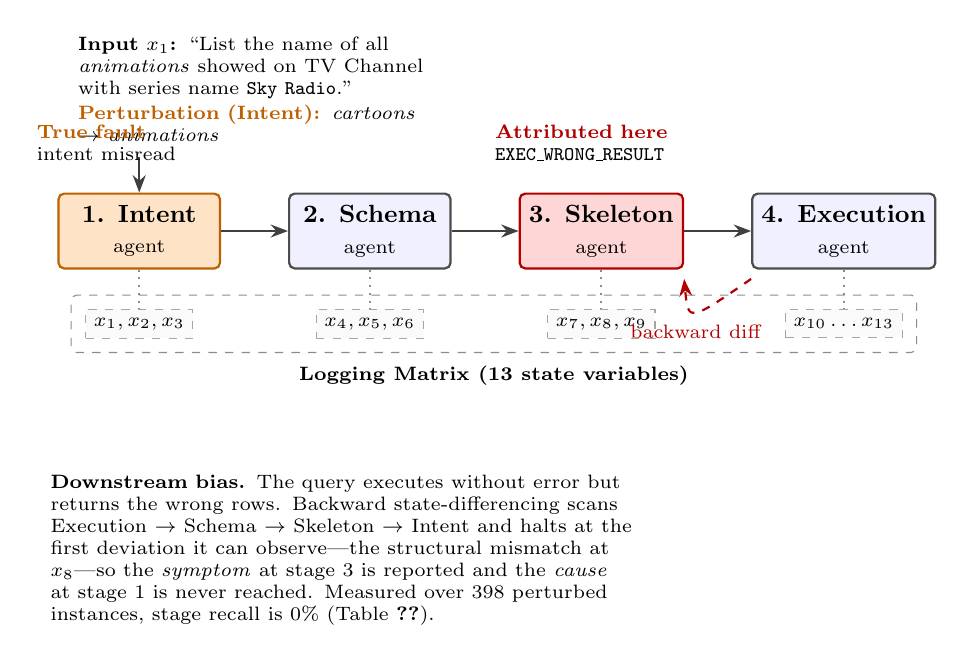
\begin{tikzpicture}[
  font=\small,
  stage/.style   = {rectangle, rounded corners=2pt, draw=black!70, thick,
                    minimum width=2.05cm, minimum height=0.95cm,
                    align=center, fill=blue!6},
  faulty/.style  = {stage, fill=orange!22, draw=orange!75!black},
  blamed/.style  = {stage, fill=red!16, draw=red!70!black},
  logbox/.style  = {rectangle, draw=black!35, dashed, inner sep=3pt,
                    align=center, font=\scriptsize, fill=black!2},
  note/.style    = {align=left, font=\scriptsize, text width=3.5cm},
  fwd/.style     = {-{Stealth[length=2.2mm]}, thick, black!75},
  back/.style    = {-{Stealth[length=2.2mm]}, thick, red!70!black, dashed}
]

% ---------- input ----------
\node[note, text width=4.4cm, anchor=west] (q) at (0,3.15)
  {\textbf{Input $x_1$:} ``List the name of all \emph{animations}
   showed on TV Channel with series name \texttt{Sky Radio}.''\\[1pt]
   \textcolor{orange!75!black}{\textbf{Perturbation (Intent):}}
   \emph{cartoons} $\rightarrow$ \emph{animations}};

% ---------- pipeline stages ----------
\node[faulty] (intent)   at (0.9,1.35) {\textbf{1. Intent}\\\scriptsize agent};
\node[stage, right=0.85cm of intent]  (schema)   {\textbf{2. Schema}\\\scriptsize agent};
\node[blamed, right=0.85cm of schema] (skeleton) {\textbf{3. Skeleton}\\\scriptsize agent};
\node[stage, right=0.85cm of skeleton](exec)     {\textbf{4. Execution}\\\scriptsize agent};

\draw[fwd] (intent)   -- (schema);
\draw[fwd] (schema)   -- (skeleton);
\draw[fwd] (skeleton) -- (exec);
\draw[fwd] ([yshift=-2pt]q.south -| intent.north) -- (intent.north);

% ---------- logging matrix ----------
\node[logbox, below=0.5cm of intent]   (l1) {$x_1,x_2,x_3$};
\node[logbox, below=0.5cm of schema]   (l2) {$x_4,x_5,x_6$};
\node[logbox, below=0.5cm of skeleton] (l3) {$x_7,x_8,x_9$};
\node[logbox, below=0.5cm of exec]     (l4) {$x_{10}\ldots x_{13}$};

\foreach \s/\l in {intent/l1, schema/l2, skeleton/l3, exec/l4}
  \draw[black!45, dotted, thick] (\s) -- (\l);

\node[draw=black!45, dashed, rounded corners=2pt, inner sep=5pt,
      fit=(l1)(l4), label={[font=\scriptsize\bfseries, yshift=-1pt]below:%
      Logging Matrix (13 state variables)}] (matrix) {};

% ---------- fault propagation ----------
\node[note, text width=2.6cm, anchor=south, font=\scriptsize]
  at ([yshift=0.28cm]intent.north)
  {\textcolor{orange!75!black}{\textbf{True fault}}\\ intent misread};

\node[note, text width=2.7cm, anchor=south, font=\scriptsize]
  at ([yshift=0.28cm]skeleton.north)
  {\textcolor{red!70!black}{\textbf{Attributed here}}\\ \texttt{EXEC\_WRONG\_RESULT}};

% ---------- backward diffing ----------
\draw[back] ([yshift=-0.12cm]exec.south west) .. controls +(-0.8,-0.55) ..
            ([yshift=-0.12cm]skeleton.south east)
  node[midway, below, font=\scriptsize, text=red!70!black, yshift=-1pt]
  {backward diff};

\node[note, text width=7.6cm, anchor=north west, font=\scriptsize]
  at (-0.35,-1.62)
  {\textbf{Downstream bias.} The query executes without error but returns the
   wrong rows. Backward state-differencing scans Execution $\rightarrow$
   Schema $\rightarrow$ Skeleton $\rightarrow$ Intent and halts at the first
   deviation it can observe---the structural mismatch at $x_8$---so the
   \emph{symptom} at stage~3 is reported and the \emph{cause} at stage~1 is
   never reached. Measured over 398 perturbed instances, stage recall is
   $0\%$ (Table~\ref{tab:confusion}).};

\end{tikzpicture}

% Requires: \usetikzlibrary{shapes.geometric, arrows.meta, positioning}
%
% Illustrates the downstream-bias mechanism: a fault injected at the Intent
% stage propagates forward and is attributed to the Skeleton stage, because
% backward state-differencing meets the symptom before the cause.

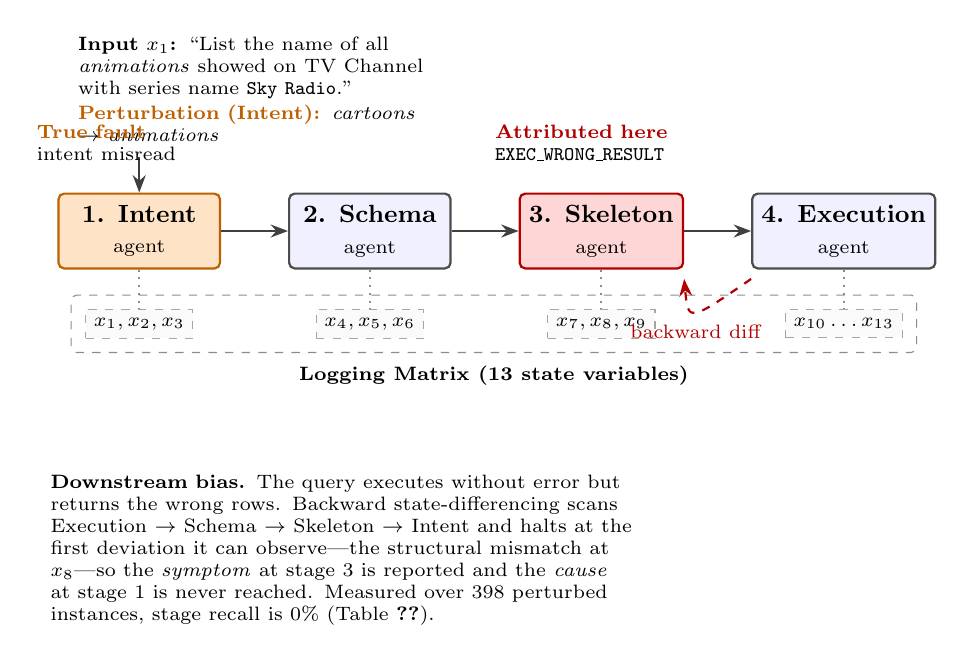
\begin{tikzpicture}[
  font=\small,
  stage/.style   = {rectangle, rounded corners=2pt, draw=black!70, thick,
                    minimum width=2.05cm, minimum height=0.95cm,
                    align=center, fill=blue!6},
  faulty/.style  = {stage, fill=orange!22, draw=orange!75!black},
  blamed/.style  = {stage, fill=red!16, draw=red!70!black},
  logbox/.style  = {rectangle, draw=black!35, dashed, inner sep=3pt,
                    align=center, font=\scriptsize, fill=black!2},
  note/.style    = {align=left, font=\scriptsize, text width=3.5cm},
  fwd/.style     = {-{Stealth[length=2.2mm]}, thick, black!75},
  back/.style    = {-{Stealth[length=2.2mm]}, thick, red!70!black, dashed}
]

% ---------- input ----------
\node[note, text width=4.4cm, anchor=west] (q) at (0,3.15)
  {\textbf{Input $x_1$:} ``List the name of all \emph{animations}
   showed on TV Channel with series name \texttt{Sky Radio}.''\\[1pt]
   \textcolor{orange!75!black}{\textbf{Perturbation (Intent):}}
   \emph{cartoons} $\rightarrow$ \emph{animations}};

% ---------- pipeline stages ----------
\node[faulty] (intent)   at (0.9,1.35) {\textbf{1. Intent}\\\scriptsize agent};
\node[stage, right=0.85cm of intent]  (schema)   {\textbf{2. Schema}\\\scriptsize agent};
\node[blamed, right=0.85cm of schema] (skeleton) {\textbf{3. Skeleton}\\\scriptsize agent};
\node[stage, right=0.85cm of skeleton](exec)     {\textbf{4. Execution}\\\scriptsize agent};

\draw[fwd] (intent)   -- (schema);
\draw[fwd] (schema)   -- (skeleton);
\draw[fwd] (skeleton) -- (exec);
\draw[fwd] ([yshift=-2pt]q.south -| intent.north) -- (intent.north);

% ---------- logging matrix ----------
\node[logbox, below=0.5cm of intent]   (l1) {$x_1,x_2,x_3$};
\node[logbox, below=0.5cm of schema]   (l2) {$x_4,x_5,x_6$};
\node[logbox, below=0.5cm of skeleton] (l3) {$x_7,x_8,x_9$};
\node[logbox, below=0.5cm of exec]     (l4) {$x_{10}\ldots x_{13}$};

\foreach \s/\l in {intent/l1, schema/l2, skeleton/l3, exec/l4}
  \draw[black!45, dotted, thick] (\s) -- (\l);

\node[draw=black!45, dashed, rounded corners=2pt, inner sep=5pt,
      fit=(l1)(l4), label={[font=\scriptsize\bfseries, yshift=-1pt]below:%
      Logging Matrix (13 state variables)}] (matrix) {};

% ---------- fault propagation ----------
\node[note, text width=2.6cm, anchor=south, font=\scriptsize]
  at ([yshift=0.28cm]intent.north)
  {\textcolor{orange!75!black}{\textbf{True fault}}\\ intent misread};

\node[note, text width=2.7cm, anchor=south, font=\scriptsize]
  at ([yshift=0.28cm]skeleton.north)
  {\textcolor{red!70!black}{\textbf{Attributed here}}\\ \texttt{EXEC\_WRONG\_RESULT}};

% ---------- backward diffing ----------
\draw[back] ([yshift=-0.12cm]exec.south west) .. controls +(-0.8,-0.55) ..
            ([yshift=-0.12cm]skeleton.south east)
  node[midway, below, font=\scriptsize, text=red!70!black, yshift=-1pt]
  {backward diff};

\node[note, text width=7.6cm, anchor=north west, font=\scriptsize]
  at (-0.35,-1.62)
  {\textbf{Downstream bias.} The query executes without error but returns the
   wrong rows. Backward state-differencing scans Execution $\rightarrow$
   Schema $\rightarrow$ Skeleton $\rightarrow$ Intent and halts at the first
   deviation it can observe---the structural mismatch at $x_8$---so the
   \emph{symptom} at stage~3 is reported and the \emph{cause} at stage~1 is
   never reached. Measured over 398 perturbed instances, stage recall is
   $0\%$ (Table~\ref{tab:confusion}).};

\end{tikzpicture}

% Requires: \usetikzlibrary{shapes.geometric, arrows.meta, positioning}
%
% Illustrates the downstream-bias mechanism: a fault injected at the Intent
% stage propagates forward and is attributed to the Skeleton stage, because
% backward state-differencing meets the symptom before the cause.

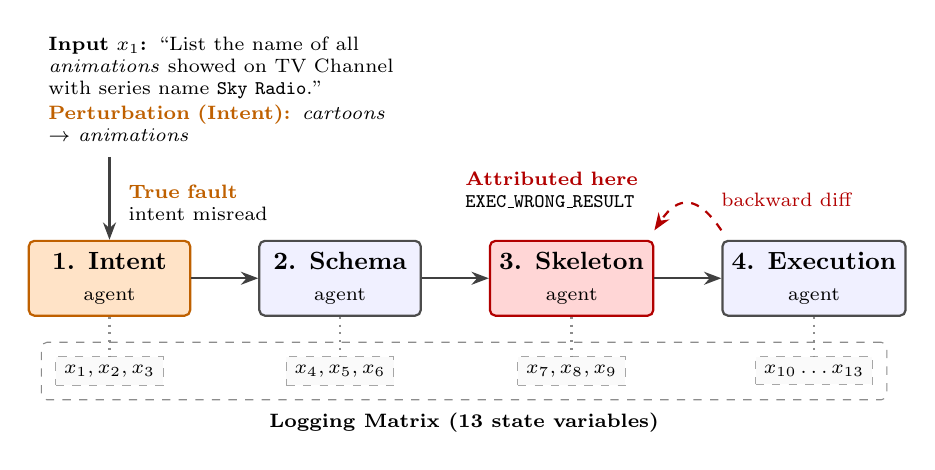
\begin{tikzpicture}[
  font=\small,
  stage/.style   = {rectangle, rounded corners=2pt, draw=black!70, thick,
                    minimum width=2.05cm, minimum height=0.95cm,
                    align=center, fill=blue!6},
  faulty/.style  = {stage, fill=orange!22, draw=orange!75!black},
  blamed/.style  = {stage, fill=red!16, draw=red!70!black},
  logbox/.style  = {rectangle, draw=black!35, dashed, inner sep=3pt,
                    align=center, font=\scriptsize, fill=black!2},
  note/.style    = {align=left, font=\scriptsize, text width=3.5cm},
  fwd/.style     = {-{Stealth[length=2.2mm]}, thick, black!75},
  back/.style    = {-{Stealth[length=2.2mm]}, thick, red!70!black, dashed}
]

% ---------- input ----------
\node[note, text width=4.4cm, anchor=west] (q) at (0,3.75)
  {\textbf{Input $x_1$:} ``List the name of all \emph{animations}
   showed on TV Channel with series name \texttt{Sky Radio}.''\\[1pt]
   \textcolor{orange!75!black}{\textbf{Perturbation (Intent):}}
   \emph{cartoons} $\rightarrow$ \emph{animations}};

% ---------- pipeline stages ----------
\node[faulty] (intent)   at (0.9,1.35) {\textbf{1. Intent}\\\scriptsize agent};
\node[stage, right=0.85cm of intent]  (schema)   {\textbf{2. Schema}\\\scriptsize agent};
\node[blamed, right=0.85cm of schema] (skeleton) {\textbf{3. Skeleton}\\\scriptsize agent};
\node[stage, right=0.85cm of skeleton](exec)     {\textbf{4. Execution}\\\scriptsize agent};

\draw[fwd] (intent)   -- (schema);
\draw[fwd] (schema)   -- (skeleton);
\draw[fwd] (skeleton) -- (exec);
\draw[fwd] ([yshift=-2pt]q.south -| intent.north) -- (intent.north);

% ---------- logging matrix ----------
\node[logbox, below=0.5cm of intent]   (l1) {$x_1,x_2,x_3$};
\node[logbox, below=0.5cm of schema]   (l2) {$x_4,x_5,x_6$};
\node[logbox, below=0.5cm of skeleton] (l3) {$x_7,x_8,x_9$};
\node[logbox, below=0.5cm of exec]     (l4) {$x_{10}\ldots x_{13}$};

\foreach \s/\l in {intent/l1, schema/l2, skeleton/l3, exec/l4}
  \draw[black!45, dotted, thick] (\s) -- (\l);

\node[draw=black!45, dashed, rounded corners=2pt, inner sep=5pt,
      fit=(l1)(l4), label={[font=\scriptsize\bfseries, yshift=-1pt]below:%
      Logging Matrix (13 state variables)}] (matrix) {};

% ---------- fault propagation ----------
\node[note, text width=2.4cm, anchor=south west, font=\scriptsize]
  at ([xshift=0.12cm,yshift=0.12cm]intent.north)
  {\textcolor{orange!75!black}{\textbf{True fault}}\\ intent misread};

\node[note, text width=2.7cm, anchor=south, font=\scriptsize]
  at ([yshift=0.28cm]skeleton.north)
  {\textcolor{red!70!black}{\textbf{Attributed here}}\\ \texttt{EXEC\_WRONG\_RESULT}};

% ---------- backward diffing ----------
\draw[back] ([yshift=0.12cm]exec.north west) .. controls +(-0.3,0.45) and +(0.3,0.45) ..
            ([yshift=0.12cm]skeleton.north east)
  node[pos=0.15, above right, font=\scriptsize, text=red!70!black]
  {backward diff};

\end{tikzpicture}
}
    \caption{The downstream-bias mechanism. A fault injected at the Intent stage
    (orange) propagates forward and yields a valid query that returns the wrong
    rows. Backward state-differencing scans from Execution upstream and halts
    at the first observable deviation, so it reports the Skeleton stage (red),
    the symptom, and never reaches the cause. Over 398 perturbed instances, stage
    recall is $0\%$ (Table~\ref{tab:confusion}).}
    \label{fig:running_example}
\end{figure}

\subsection{The Logging Matrix}

Each run is stored as a structured JSON \texttt{PipelineLogEntry} holding 13
state variables $x_1,\dots,x_{13}$ (Table~\ref{tab:logging}). Coupled with
lightweight detectors, they form the attribution
mechanism~\cite{zhang2025which}.

\begin{table}[t]
\centering
\caption{State variables logged per pipeline run.}
\label{tab:logging}
\small
\begin{tabular}{lp{10cm}}
\toprule
Var. & Content \\
\midrule
$x_1$  & Input: question, \texttt{db\_id}, full schema, metadata \\
$x_2$  & External knowledge: domain hints and constraints \\
$x_3$  & Clarified intent: refined intent, subtasks, detected conditions \\
$x_4$, $x_5$ & Full schema; filtered schema after pruning \\
$x_6$  & Schema alignment: token-to-schema mapping with confidence \\
$x_7$  & Query plan: required joins, aggregations, reasoning trace \\
$x_8$, $x_9$ & SQL skeleton with clause placeholders; candidate SQLs \\
$x_{10}$, $x_{11}$ & Final SQL sent to the DBMS; result set or engine error \\
$x_{12}$, $x_{13}$ & Failure analysis (label, explanation, fix); repaired SQL \\
\bottomrule
\end{tabular}
\end{table}

\subsection{Backward Differencing}

To attribute a failure, we start from the outcome $x_{11}$ and compare
backward through the states until the first significant deviation
(Algorithm~\ref{alg:backdiff}). This algorithm produced every label in this
paper. The matrix supports further detectors that write diagnostic fields into
$x_{12}$ without affecting the label: an alignment-confidence band
$[0.30,0.55]$ on $x_6$, calibrated on 50 held-out development queries disjoint
from both data sets; a self-consistency score over the candidates $x_9$; a
check of $x_3$ for constraints absent from $x_1$ and
$x_2$~\cite{ding_ambisql_2025}; and a repair-regression check comparing
$x_{13}$ with $x_9$. No result below depends on them.

\begin{algorithm}[t]
\caption{Backward differencing for root-cause attribution}
\label{alg:backdiff}
\begin{algorithmic}[1]
\REQUIRE Log entry $(x_1,\ldots,x_{13})$, gold SQL $q^*$
\ENSURE Root-cause label $L$
\IF{$x_{11}$ contains a DB engine error}
    \STATE \textbf{return} $L \leftarrow \texttt{EXECUTION\_SYNTAX}$
\ENDIF
\IF{$\text{result}(x_{10}) \neq \text{result}(q^*)$}
    \IF{$x_5$ lacks tables/columns required by $q^*$}
        \STATE \textbf{return} $L \leftarrow \texttt{SCHEMA\_MISSING}$
    \ENDIF
    \IF{$x_6$ maps tokens to non-existent schema elements}
        \STATE \textbf{return} $L \leftarrow \texttt{SCHEMA\_HALLUCINATION}$
    \ENDIF
    \IF{clauses in $x_8$ are absent from $x_{10}$}
        \STATE \textbf{return} $L \leftarrow \texttt{SKELETON\_STRUCTURAL}$
    \ENDIF
    \IF{$x_3$ omits conditions present in $x_1$}
        \STATE \textbf{return} $L \leftarrow \texttt{INTENT\_MISSING\_CONDITION}$
    \ENDIF
\ENDIF
\STATE \textbf{return} $L \leftarrow \texttt{UNKNOWN}$
\end{algorithmic}
\end{algorithm}

\subsection{Ordering Sensitivity and Downstream Bias}
\label{sec:bias_design}

Algorithm~\ref{alg:backdiff} checks its conditions in a fixed downstream-first
order: execution, schema, skeleton, intent. The order is forced by the
pipeline: only execution yields an unambiguous, externally verifiable signal,
while upstream states are latent and can be judged only by proxy tests over
$x_3$, $x_5$ and $x_6$. Model the pipeline as a chain
$s_1\to s_2\to s_3\to s_4$ in which a fault at $s_i$ perturbs every $x_j$ with
$j>i$, and let $b_k$ be the detector for stage $k$. A procedure that returns
the first stage in the order $(4,2,3,1)$ whose detector fires gives
\begin{equation}
P(\hat{L}=s \mid \text{fault at } s) = P(b_s \text{ fires})\prod_{k \prec s}\left[1 - P(b_k \text{ fires})\right],
\label{eq:bias}
\end{equation}
where $k\prec s$ ranges over the branches checked before $s$. Both factors work
against upstream stages: forward propagation raises the firing rate of
downstream detectors, and the intent branch is checked last. The attributed
distribution $P(\hat{L})$ is therefore a biased functional of the true fault
distribution, not an estimator of it.

Two design choices compound this. The intent branch fires only on an explicit
\texttt{is\_ambiguous} flag on $x_3$ or on a clarified question shorter than
$60\%$ of the original; neither triggers for a fluent paraphrase that the
intent agent confidently misreads. The schema branch requires a gold table to
be absent from $x_5$, so an agent that picks a \emph{plausible but wrong} table
passes. For the perturbations used here, the intent factor of
Eq.~\eqref{eq:bias} is thus close to zero \emph{by construction}, so the
intent recall we report is largely a property of how that branch was written
and only partly of the ordering. We separate the two claims in
Section~\ref{sec:bias_results} and treat the heuristic as an object of
measurement rather than a trusted instrument.

\section{Experiments and Results}
\label{sec:experiments}

\subsection{Data and Setup}
\label{sec:benchmark}

Two disjoint collections are used and never pooled. \textbf{(i)~The
distribution set} is all $7{,}000$ instances of the Spider~\cite{yu_spider_2018}
\emph{training} split, run end-to-end for the stage distribution of
Section~\ref{sec:failure_dist}. The training split is Spider's largest, which
matters because the quantity of interest is a distribution over failure
categories, and it keeps this set disjoint from the perturbation set. Its
questions are plausibly in the backbone's pretraining data, so the EX rates
below should not be compared with leaderboard figures. \textbf{(ii)~The
perturbation set} contains $400$ instances from the Spider \emph{validation}
split and Spider-Syn~\cite{gan_spider_syn_2021}, used only in
Section~\ref{sec:bias_results} (Table~\ref{tab:benchmark}).

\begin{table}[t]
\centering
\caption{Perturbation benchmark composition.}
\label{tab:benchmark}
\small
\begin{tabular}{llcc}
\toprule
Source & Perturbation & \# & Target stage \\
\midrule
Spider validation & Schema proxy      & 200 & Schema \\
Spider-Syn        & Intent paraphrase & 200 & Intent \\
\midrule
\multicolumn{2}{l}{\textbf{Total} (398 unique)} & \textbf{400} & -- \\
\bottomrule
\end{tabular}
\end{table}

Ground truth is fixed \emph{by construction}. A \emph{schema-proxy} instance
keeps the question and gold SQL and adds to the catalogue a distractor table
whose name is lexically close to a table of the gold query and whose columns
are copied from it, so the schema agent must choose between two similar
candidates. The construction \emph{adds} a distractor rather than removing the
gold table, which matters below because \texttt{SCHEMA\_MISSING} fires only on
absence. An \emph{intent-paraphrase} instance keeps the database and gold SQL
and replaces the question with its Spider-Syn synonym substitution, which
preserves the gold SQL~\cite{gan_spider_syn_2021}. Two schema-proxy items are
duplicate \texttt{(db\_id, question)} pairs, leaving $200$ intent and $198$
schema instances. Construction-time labels certify where a fault was
\emph{injected}, not that the pipeline failed there, but they are not produced
by the reasoning being evaluated and so cannot inherit its biases; a heuristic
scored against labels derived from its own signals would be scored against
itself.

All runs use gpt-4o-mini as the backbone for every agent and execute the
predicted SQL on local SQLite databases. The pipeline reaches $62.21\%$ EX
before rerun ($4{,}066/6{,}536$ completed runs) and $70.10\%$ after
self-correction ($4{,}754/6{,}782$; rerun also recovers runs that had timed
out). It is a diagnostic testbed, not a performance-optimised system. We do
not report exact match: our implementation compared normalised strings rather
than Spider's clause-level Exact Set Match and returned $0.00\%$, a property of
the comparison, not of the model. Of the $7{,}000$ runs, $218$ ended in API or
network timeouts after rerun ($464$ before). These carry no information about
pipeline reasoning, so they are excluded from the taxonomy and all
denominators but listed in Table~\ref{tab:failures}.

\subsection{Framework-Attributed Stage Distribution (RQ1)}
\label{sec:failure_dist}

Table~\ref{tab:failures} gives the stage labels before and after rerun. We call
it \emph{framework-attributed} deliberately: Section~\ref{sec:bias_results}
shows that it cannot be read as the pipeline's fault distribution.

\begin{table}[t]
\centering
\caption{Framework-attributed stage distribution before and after rerun. Rates
are over completed runs; infrastructure failures are listed separately.}
\label{tab:failures}
\small
\begin{tabular}{lrrrr}
\toprule
& \multicolumn{2}{c}{Pre-rerun} & \multicolumn{2}{c}{Post-rerun} \\
Attributed stage & \# & \% & \# & \% \\
\midrule
Intent                 & 0       & 0.00  & 0       & 0.00 \\
Schema linking         & 164     & 2.51  & 163     & 2.40 \\
Skeleton / structural  & 1{,}669 & 25.54 & 1{,}845 & 27.20 \\
Execution / syntax     & 637     & 9.75  & 20      & 0.29 \\
Correct (EX pass)      & 4{,}066 & 62.21 & 4{,}754 & 70.10 \\
\midrule
\textbf{Completed}     & \textbf{6{,}536} & \textbf{100} & \textbf{6{,}782} & \textbf{100} \\
Excluded: API/network timeout & 464 & -- & 218 & -- \\
\textbf{Total runs}    & \textbf{7{,}000} & & \textbf{7{,}000} & \\
\bottomrule
\end{tabular}
\end{table}

\noindent\textbf{Execution / syntax} falls from $637$ to $20$ runs after
self-correction. For example, a query using \texttt{ILIKE}, which SQLite does
not support, raises \texttt{near "ILIKE": syntax error} and is repaired on
rerun. \textbf{Skeleton / structural} rises from $1{,}669$ to $1{,}845$ runs,
because repaired syntax errors expose underlying semantic errors; for ``How
many heads of the departments are older than 56?'' the skeleton agent inserts
a redundant \texttt{JOIN management} and returns 3 instead of the correct
count. \textbf{Schema linking} covers $163$ runs ($140$ missing table, $23$
hallucinated element); for a question on farm competitions, the schema agent
prunes the \texttt{farm} table. \textbf{Intent} is exactly zero across all
$7{,}000$ runs. Given that $200$ perturbation instances were built to induce
intent failures, a zero is not plausibly a property of the intent agent; it is
the signature of the ordering effect of Section~\ref{sec:bias_design}.

Stratifying the post-rerun labels by query difficulty (tiers assigned by a
structural heuristic over the gold query, not Spider's official labels) gives
the same shape at every tier: Skeleton dominates, peaking at Medium
($1{,}033$); Execution stays near zero ($2$, $12$, $6$, $0$ from Easy to Extra
Hard); Schema stays low ($43$, $86$, $33$, $1$); and Intent is zero throughout.
Read at face value, Skeleton accounts for $90.98\%$ of attributed failures
($1{,}845/2{,}028$), and execution-only repair would address $0.99\%$ of them
($20/2{,}028$). The second figure survives scrutiny, because these are runs
the DB engine itself rejected and the count does not depend on the heuristic.
The first does not yet: the claim that repair belongs at the skeleton stage
rests entirely on $1{,}845$ being a count of skeleton faults. We now test that
premise.

\subsection{Measuring the Heuristic (RQ2)}
\label{sec:bias_results}

We run the $398$ unique perturbation instances through the pipeline and
compare the emitted label with the injected stage (Table~\ref{tab:confusion}).

\begin{table}[t]
\centering
\caption{Attribution of injected faults. Rows: stage stressed by construction;
columns: stage reported by the heuristic. \emph{Passed} counts instances
answered correctly despite the perturbation and is excluded from recall.}
\label{tab:confusion}
\small
\begin{tabular}{lccccc}
\toprule
& \multicolumn{4}{c}{Attributed stage} & \\
Injected at & Intent & Schema & Skeleton & Exec. & Passed \\
\midrule
Intent ($n{=}200$) & \textbf{0} & 1 & 59 & 38 & 102 \\
Schema ($n{=}198$) & 0 & \textbf{0} & 33 & 21 & 144 \\
\midrule
\multicolumn{6}{l}{Recall on failed instances: Intent $0/98=\mathbf{0.00\%}$;
Schema $0/54=\mathbf{0.00\%}$} \\
\bottomrule
\end{tabular}
\end{table}

\noindent\textbf{(1) Stage recall is zero.} None of the $98$ failed
intent-perturbed instances was attributed to Intent ($0/98$; Wilson $95\%$ CI
$[0.0\%,3.8\%]$), and none of the $54$ failed schema-perturbed instances to
Schema ($0/54$; CI $[0.0\%,6.6\%]$). The two zeros have different causes. The
intent zero is largely mechanical: neither gating condition of the intent
branch can fire on a fluent paraphrase, so it was predictable from the
algorithm, and the measurement confirms rather than discovers it. The schema
zero is the informative one: the distractor leaves the gold table in place,
so \texttt{SCHEMA\_MISSING} is \emph{correct} not to fire, and the heuristic has
no detector for the failure the perturbation actually induces, namely picking
a plausible but wrong table. The small $n$ of the schema row should temper how
strongly this zero is read.

\noindent\textbf{(2) Labels are biased downstream, whatever the injection.}
All but one of the $152$ failures ($151$) were attributed to Skeleton or
Execution, the two stages scanned first or nearest the outcome, as
Eq.~\eqref{eq:bias} predicts. Among
failures, intent-injected faults were labelled Skeleton in $60.2\%$ and
Execution in $38.8\%$ of cases; schema-injected faults in $61.1\%$ and
$38.9\%$. On the Skeleton/Execution cells, a $\chi^2$ test gives
$\chi^2=0.001$, $p=0.97$. A large $p$-value is not evidence of independence:
with $n=151$ the $95\%$ CI on the difference in Skeleton share spans about
$\pm16$ points. The defensible statement is that at this sample size the
heuristic's output carries \emph{no detectable} signal about fault provenance,
not that the signal is provably zero; an equivalence test against a
pre-registered margin would be needed for the stronger claim.

\noindent\textbf{(3) Perturbations often fail to perturb.} $246$ of $398$
instances ($61.8\%$) were answered correctly despite the perturbation, so
synonym substitution and table proxies are largely within the tolerance of a
gpt-4o-mini pipeline. This bounds the sensitivity of the benchmark and raises
a construct-validity threat: among the $38.2\%$ that failed, construction
certifies where the fault was injected, not that the pipeline failed there.

\noindent\textbf{Consequence for Table~\ref{tab:failures}.} With zero recall at
two of four stages, the $27.20\%$ skeleton figure is an upper bound that
demonstrably absorbs injected intent and schema faults, and the $0.00\%$
intent figure carries no information. We keep the table, labelled
framework-attributed, and withdraw the claim of an earlier version of this
work that skeleton reasoning is empirically the dominant failure source in MAS
Text-to-SQL: an instrument that cannot separate a skeleton fault from an
intent fault cannot support it.

\noindent\textbf{Why we report this rather than repair it.} Reordering the
algorithm upstream-first would, by the mirror-image mechanism, over-attribute
to intent and trade one bias for another. Eq.~\eqref{eq:bias} suggests a second
repair: the product term vanishes if every detector is evaluated and stages
are ranked by independent evidence strength. Removing precedence does not,
however, add a detector for a confidently misread paraphrase or for a
plausible but wrong table, which are the two failures our benchmark induces,
so we do not expect it to recover the signal missing here. The deeper
obstacle is that single-pass differencing infers a cause from a downstream
symptom, and cascading failure does not admit that inversion without
re-executing the pipeline under controlled changes or an independent judge
such as the human annotation behind MAST~\cite{cemri_mast_2025}. The
transferable contribution is therefore the measurement protocol of this
section, which is cheap, needs only construction-time ground truth, and
applies to the attribution methods of Section~\ref{sec:related}.

\section{Limitations}
\label{sec:limitations}

\noindent\textbf{One heuristic, one pipeline.} This suffices to invalidate our
own distribution and to demonstrate the protocol, but not to characterise
backward state-differencing as a class, and we do not claim the downstream
bias is architectural. Finding~(1) traces both zeros to specific branches of
Algorithm~\ref{alg:backdiff}, so a different implementation, pipeline or
backbone may well reach non-zero recall.

\noindent\textbf{Ground-truth validity.} Every recall figure assumes that a
perturbed-at-$X$ instance which fails did fail at $X$; with a $61.8\%$ pass
rate this is a live concern that independent human annotation of the $152$
failures, with inter-annotator agreement, would settle. It has not been run
on this set.

\noindent\textbf{Backbone, data and reproducibility.} All $7{,}000$ runs use
gpt-4o-mini on Spider with SQLite, so neither the distribution nor the
measured bias has been shown to transfer to other backbones or benchmarks.
The per-run logs of the $398$ perturbation runs were not retained, so
alternative attribution rules cannot be re-scored on them; the released code
is meant to prevent this recurring. BIRD would reuse the Logging Matrix
unchanged, with its \texttt{evidence} field filling the dormant $x_2$ slot,
whereas Spider~2.0 and conversational benchmarks need engines and dialogue
state the matrix does not model.

\section{Conclusion}
\label{sec:conclusion}

High end-to-end accuracy in MAS Text-to-SQL hides the errors of individual
agents, and without intermediate logging self-correction patches symptoms
rather than causes. Our Logging Matrix makes the four-stage pipeline
observable, but observability proved insufficient for attribution. On
$7{,}000$ Spider runs one claim holds regardless of attribution quality: after
self-correction only $20$ failures are rejected by the DB engine, so
execution-level repair addresses under $1\%$ of what goes wrong. The stronger
claim, that skeleton reasoning is the dominant failure source, depends on the
heuristic, and scoring it on $398$ perturbations with construction-time ground
truth gives $0\%$ stage recall for injected intent and schema faults and
indistinguishable label distributions. We therefore report the distribution
as framework-attributed and withdraw the dominance claim.

We see the negative result as the more useful contribution. Automated failure
attribution tools are spreading with little independent
validation~\cite{zhang2025which,cemri_mast_2025}, and a heuristic that emits
confident, well-formed stage labels with no detectable signal about the true
fault stage is a specific hazard: its output looks like evidence. Injecting
faults at known stages, scoring recall and publishing the confusion matrix is
a cheap guard. Future work will build stronger perturbations that break the
pipeline more often, add human annotation of the failing instances, and repeat
the measurement with further backbones to see which parts of this result hold
beyond the present configuration.

\bibliographystyle{splncs04}
\bibliography{failureAttribution}

\end{document}
